\documentclass[letterpaper,10pt]{article}
\usepackage[T1]{fontenc}
\usepackage[utf8]{inputenc}
\usepackage{lmodern}
\usepackage[english]{babel}
\usepackage{amsmath}
\usepackage{amsfonts}
\usepackage{fullpage}
\usepackage{graphicx}
\usepackage{enumerate}
\usepackage{setspace}
\usepackage{ amssymb }

% http://www.maths.tcd.ie/~dwilkins/LaTeXPrimer/Theorems.html
\newtheorem{theorem}{Theorem}[section]
\newtheorem{lemma}[theorem]{Lemma}
\newtheorem{proposition}[theorem]{Proposition}
\newtheorem{corollary}[theorem]{Corollary}

\newenvironment{proof}[1][Proof]{\begin{trivlist}
\item[\hskip \labelsep {\bfseries #1}]}{\end{trivlist}}
\newenvironment{definition}[1][Definition]{\begin{trivlist}
\item[\hskip \labelsep {\bfseries #1}]}{\end{trivlist}}
\newenvironment{example}[1][Example]{\begin{trivlist}
\item[\hskip \labelsep {\bfseries #1}]}{\end{trivlist}}
\newenvironment{remark}[1][Remark]{\begin{trivlist}
\item[\hskip \labelsep {\bfseries #1}]}{\end{trivlist}}

\newcommand{\qed}{\nobreak \ifvmode \relax \else
      \ifdim\lastskip<1.5em \hskip-\lastskip
      \hskip1.5em plus0em minus0.5em \fi \nobreak
      \vrule height0.75em width0.5em depth0.25em\fi}


% \def\pball{\mathrel{%
%     \mathchoice{\PBALL}{\PBALL}{\scriptsize\PBALL}{\tiny\PBALL}%
% }}
% \def\PBALL{{%
%     \setbox0\hbox{B}%
%     \rlap{\hbox to \wd0{\hss|\hss}}\box0
% }}

\allowdisplaybreaks
\newcommand{\tinyquot}[1]{\begin{center}{\footnotesize #1}\end{center}}
\newcommand*{\QEDA}{\hfill\ensuremath{\blacksquare}}
\addtolength{\belowdisplayskip}{-25mm}
\begin{document}
\title{Assignment 5 - MAT257}
\author{David Knott \\  Student \#999817685}
\date{October 18, 2013}
\maketitle
\begin{enumerate}
	\item Munkres \S 2.6, Question 1

	Let $B = [0, 0]$. $B$ is the derivative of $f$ at $(0, 0)$ if the following holds:
	$$ \frac{f(h) - f(0) - B \cdot h}{|h|} \to 0 \text{ as } h \to 0$$
	After expending out the terms we find that the above is equivalent to the following:
	$$ \frac{|h_1 \cdot h_2|}{|h|} \to 0 \text{ as } h \to 0$$
	This can be proven with a simple delta-epsilon proof. Given any $\epsilon > 0$, if we take $\delta = \epsilon$ then given $k \in C(0, \delta)$ assuming that $k_1 \geq k_2$ then for some $0 \leq \gamma \leq 1$ we have $k_1 = \gamma k_2$. Also, because $k_1 \geq k_2$ then $|k| = k_1$. This implies the following:
	$$\frac{|k_1 \cdot k_2 |}{|k|} = \frac {\gamma|k_1| \cdot |k_1|}{|k_1|} = \gamma|k_1|$$
	Since $|k| < \delta$ this implies $\gamma|k_1| < \delta$. Since $\delta = \epsilon$ we have that $\frac{|k_1 \cdot k_2 |}{|k|} < \epsilon$. The case when $k_2 \geq k_1$ is essentially the same.

	The function is not of class $C_1$ for any neighborhood of $0$, since for any $\epsilon > 0$ we have $(0, \epsilon) \in C(0, 2\epsilon)$. If we take $D_1 f((0, \epsilon)) = f'((0, \epsilon); e_1)$ then we must evaluate the limit:
	$$ \lim_{t \to 0} \frac{f((0, \epsilon) + te_1) - f((0, \epsilon))}{t} = \lim_{t \to 0} \frac{|t\epsilon|}{t} = \lim_{t \to 0} \text{sgn}(t) \epsilon$$
	Which doesn't exist since epsilon is positive and the sign of $t$ does not converge to any value at zero. This means for any neighborhood of $0$ there exists a point of discontinuity in the 1st partial derivative. Therefore no neighborhood around $0$ is of class $C_1$.

	\item Munkres \S 2.6, Question 2

	\begin{enumerate}
		\item Note that $f'(0) = \lim_{t \to 0} \frac{f(0+t) - f(0)}{t} = \lim_{t \to 0} \frac{t^2 \sin(1/t)}{t} = \lim_{t \to 0} t \sin(1/t)$. Since sine is bounded and $t$ goes to zero, by the squeeze theorem the whole limit goes to zero. Therefore $f'(0) = 0$.

		\item Since $t \neq 0$ we can apply the chain rule and the product rule to yield $f'(t) = 2t \sin(1/t) - \cos(1/t)$

		\item If $f'$ is continuous then $\lim_{t \to 0} f'(t) = 0$. However, if $\epsilon = 1/2$ then for any $\delta > 0$ there exists an $|x| < \delta$ such that $|2x \sin(1/x) - \cos(1/x)| > \epsilon$. This is because if we take $x$ small enough the term $|2x \sin(1/x)|$ becomes negligible, but $|\cos (1/x)|$ is still greater than $1/2$.

		\item Since the derivative is not continuous at $0$ the function is differentiable but not of class $C_1$
	\end{enumerate}

	\item Munkres \S 2.6, Question 4

	Logically I'm parsing this problem like so:
	$$ \exists \delta > 0 . \exists \epsilon > 0 . \forall j \in [1, m] . \forall m \in C(a,\delta) . D_j f(m) \text{ exists}\wedge |D_j f(m)| < \epsilon \implies f \text{ is continuous at } a $$
	Which is the pedantic way to say that there's a delta sized neighborhood around $a$ such that all the partial derivatives exist and are bounded by some epsilon. I intent to prove the contrapositive, which looks like so:
	$$  f \text{ is discontinuous at } a  \implies \forall \delta > 0 . \forall \epsilon > 0 . \exists j \in [1, m] . \exists m \in C(a,\delta) . D_j f(m) \text{ doesn't exist}\vee |D_j f(m)| \geq \epsilon $$
	Which translates to: if $f$ is discontinuous at $a$ then for any neighborhood around $a$ there is a point in the neighborhood where a partial derivative doesn't exist or given any epsilon there's a point in the neighborhood where a partial derivative's magnitude is greater than that epsilon.

	So assuming that $f$ is discontinuous at $a$, there are three possibilities for the behavior of $f$ around $a$:
	\begin{enumerate}[i.]
		\item The discontinuity of $f$ at $a$ is a removable discontinuity. Either it doesn't exist or it's a value that's unequal to the limit as $h \to a$. In this case the derivative may be bounded, but it won't exist at $a$.
		\item The discontinuity of $f$ at $a$ is a jump discontinuity. In this case limits approaching $a$ from different directions or paths will exist but yield opposing numbers. The derivative may be bounded, but it won't exist at $a$ for this reason.
		\item The discontinuity of $f$ at $a$ is an asymptotic discontinuity, which is to say for any neighborhood around $a$ and any number $\gamma > 0$ there's an $m$ in that neighborhood such that $|f(m)| > \gamma$. In this case the derivative is not bounded nor does it exist at $a$, so both of the conditions are satisfied.
	\end{enumerate}

	This covers all the cases, and each one implies the consequent. Since this proves the contrapositive, the original implication follows.

	\item Munkres \S 2.6, Question 10

	\begin{enumerate}
		\item  Since the function is zero when $x$ or $y$ are zero, the partial derivatives at zero will both be zero. This is because when computing the partials we will be essentially be computing the derivative of a constant function.
		\item Consider the following evaluated limits:
		\begin{align*}
		D_1 f(x, y) & = \lim_{t \to 0} \frac{1}{t} \Bigg( \frac{(x+t) y ((x+t)^2 - y^2)}{(x+t)^2 + y^2} - \frac{x y (x^2 - y^2)}{x^2 + y^2} \Bigg) \\
		 & = y\frac{x^4 + 4x^2 y^2 - y^4}{x^4+2 x^2 y^2+y^4} \\
		D_2 f(x, y) & = \lim_{t \to 0} \frac{1}{t} \Bigg( \frac{(y+t) x (x^2 - (y+t)^2)}{x^2 + (y+t)^2} - \frac{x y (x^2 - y^2)}{x^2 + y^2} \Bigg) \\
		 & = x\frac{x^4 - 4x^2 y^2 - y^4}{x^4+2 x^2 y^2+y^4}
		\end{align*}
		\item Because the partial derivatives are a component of $\mathbb{R}^2$ multiplied by a bounded function (the polynomials of the rational functions have equal degrees) then they will be continuous for all $x \in \mathbb{R}^2$, therefore the function is of class $C_1$.
		\item 
	\end{enumerate}

	\item Munkres \S 2.7, Question 1

	From the chain rule, we have that if $f : \mathbb{R}^n \to \mathbb{R}^m$ and $g : \mathbb{R}^m \to \mathbb{R}^p$ then for some point $a \in \mathbb{R}^n$, if $f(a) = b$ then $D(g \circ f)(a) = Dg(b) \cdot Df(a)$

	Given the functions and information posed by this question, $D(g \circ f)(0) = Dg((1,2)) \cdot Df(0)$ Where $Df(0)$ is the matrix:
	\[ \left( \begin{array}{ccc}
		1 & 2 & 3 \\
		0 & 0 & 1 \end{array} \right)\]
	$g$ is differentiable because it is the sum and product of differentiable functions. To find $Dg((1,2))$ we must find the partial derivatives for each component function at $(1,2)$ to get the derivative matrix. Note the definition of the component functions:
	\begin{align*}
		g_1((x,y)) & = x + 2y + 1 \\
		g_2((x,y)) & = 3xy
	\end{align*}
	And after a bit of limit evaluation, we find the derivatives:
	\begin{align*}
		g_1'((1,2)) & = [\; 1 \quad 2 \;] \\
		g_2'((1,2)) & = [\; 6 \quad 3 \;]
	\end{align*}
	Which makes $Dg((1,2))$ the following matrix:
	\[ \left( \begin{array}{cc}
		1 & 2 \\
		6 & 3 \end{array} \right)\]
	Multiplying $Dg((1,2))$ by $Df(0)$ yields $D(g \circ f)(0)$ which is the following:
	\[ \left( \begin{array}{ccc}
		1 & 2 & 5 \\
		6 & 12 & 21 \end{array} \right)\]

	\item Additional Work, Question 1

	\begin{enumerate}
		\item Graphs generated with Wolfram Mathematica 9. Z axis is vertical, while the X and Y axes are horizontal.
		\begin{figure}[ht]
			\begin{minipage}[b]{0.30\linewidth}
				\centering
				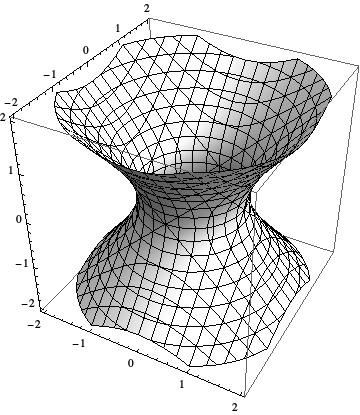
\includegraphics[width=\textwidth]{images/-1.jpeg}
				\caption{$\Sigma_{-1}$}
				\label{fig:figure1}
			\end{minipage}
			\hspace{0.3cm}
			\begin{minipage}[b]{0.30\linewidth}
				\centering
				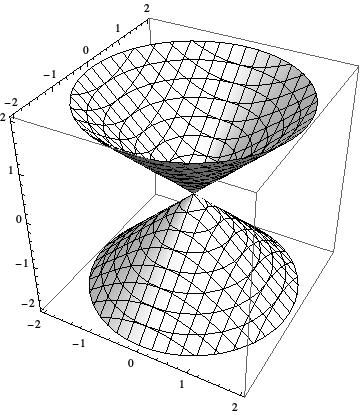
\includegraphics[width=\textwidth]{images/0.jpeg}
				\caption{$\Sigma_0$}
				\label{fig:figure2}
			\end{minipage}
			\hspace{0.3cm}
			\begin{minipage}[b]{0.30\linewidth}
				\centering
				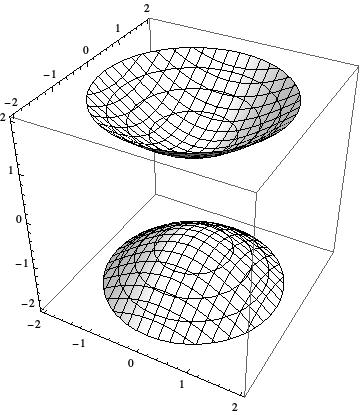
\includegraphics[width=\textwidth]{images/1.jpeg}
				\caption{$\Sigma_1$}
				\label{fig:figure2}
			\end{minipage}
		\end{figure}

		Commands:
		\begin{enumerate}[i.]
			\item $\Sigma_{-1}$:
			{\tt Show[ContourPlot3D[
  z\verb|^|2 - x\verb|^|2 - y\verb|^|2 == -1, \{x, -2, 2\}, \{y, -2, 2\}, \{z, -2, 2\}], 
 Lighting -> "Neutral"] }
			\item $\Sigma_{0}$:
			{\tt Show[ContourPlot3D[
  z\verb|^|2 - x\verb|^|2 - y\verb|^|2 == 0, \{x, -2, 2\}, \{y, -2, 2\}, \{z, -2, 2\}], 
 Lighting -> "Neutral"] }
			\item $\Sigma_{1}$:
			{\tt Show[ContourPlot3D[
  z\verb|^|2 - x\verb|^|2 - y\verb|^|2 == 1, \{x, -2, 2\}, \{y, -2, 2\}, \{z, -2, 2\}], 
 Lighting -> "Neutral"] }
		\end{enumerate}
		\item $\nabla f (x,y,z) = (-2x, -2y, 2z)$ because $\nabla f = (D_1 f)e_1 + (D_2 f)e_2 + (D_3 f)e_3$ and: 
		\begin{align*}
			D_1 f (x,y,z) & = -2x \\
			D_2 f (x,y,z) & = -2y \\ 
			D_3 f (x,y,z) & = 2z
		\end{align*}
		For the points $e_1, e_2, e_3$, $\nabla f$ takes the following values:
		\begin{align*}
			\nabla f (e_1) & = -2 e_1 \\
			\nabla f (e_2) & = -2 e_2 \\ 
			\nabla f (e_3) & = 2 e_3
		\end{align*}
		If $\nabla f(x, y, z) = (-2x, -2y, 2z) = 0$ then $(x, y, z) = 0$. The corresponding level set of this point is $\Sigma_0$. A special feature about this level set is it's the only one that contains a point that has a gradient of zero. 
		\item 
		\item 
		\item 
		\item 
	\end{enumerate}


\end{enumerate}
\end{document}
